% !TEX root = main.tex
% ============================================================================
% CHAPTER 4: IMPLEMENTATION AND RESULTS ANALYSIS
% ============================================================================

\chapter{نتایج و تجزیه و تحلیل}

\section{مقدمه}
در این فصل، نتایج پیاده‌سازی عملی الگوریتم پیشنهادی رمزنگاری تصویر ارائه و به‌طور دقیق تحلیل می‌شود. برای ارزیابی عملکرد، آزمایش‌های تجربی بر روی تصاویر رنگی استاندارد انجام شده و نتایج از جنبه‌های امنیتی، آماری و محاسباتی بررسی شده است. هدف این فصل، اعتبارسنجی عملی الگوریتم و نمایش کارایی آن در حفظ محرمانگی اطلاعات، معکوس‌پذیری کامل و مقاومت در برابر حملات رایج رمزنگاری تصویر است.

\section{مجموعه داده آزمایشی و تنظیمات محیط اجرای الگوریتم}
برای تضمین مقایسه‌پذیری، تحلیل‌ها بر روی چهار تصویر شناخته‌شده از مجموعه \lr{USC-SIPI} شامل \lr{Tree}، \lr{Peppers}، \lr{Baboon} و \lr{Airplane} انجام شده است. این تصاویر به دلیل تنوع ساختاری در بافت، تغییرات رنگی، جزئیات لبه‌ها و توزیع پیکسل‌ها، معیار مناسبی برای ارزیابی کیفیت الگوریتم‌های رمزنگاری تصویر هستند.

محیط اجرایی استاندارد و قابل بازتولید، شامل موارد زیر است:
\begin{itemize}
    \item \lr{Python 3.11} برای پردازش داده
    \item کتابخانه‌های علمی \lr{SciPy}، \lr{OpenCV}، و \lr{NumPy}
    \item پردازنده: \lr{Intel Core i7}
    \item بدون \lr{GPU}
\end{itemize}

این تنظیمات امکان تحلیل عملکرد الگوریتم در شرایط واقعی را فراهم می‌کند.

\section{تحلیل بصری خروجی‌های رمزنگاری}
نتایج رمزنگاری و رمزگشایی تصاویر آزمایشی در شکل \ref{fig:visual_results} ارائه شده است. این خروجی‌ها سه نکته اساسی را نشان می‌دهند:
\begin{enumerate}
    \item تصاویر رمزشده کاملاً نویزی هستند و هیچ ویژگی بصری قابل تشخیص ندارند. این ویژگی یکی از شاخص‌های مهم امنیتی است.
    \item تصاویر بدون خطا رمزگشایی می‌شوند و تصویر رمزگشایی‌شده با تصویر اصلی برابر است. این نشان می‌دهد الگوریتم هیچ تخریب داده‌ای ایجاد نمی‌کند.
    \item تغییرات رنگی کاملاً حذف شده‌اند و ترکیب جایگشت و انتشار مانع بازیابی هرگونه نشانه رنگی از تصویر اولیه می‌شود.
\end{enumerate}

این نتایج صحت عملکرد و پایداری الگوریتم را تأیید می‌کند.

\begin{figure}[htbp]
    \centering
    \begin{subfigure}{0.31\textwidth}
        \centering
        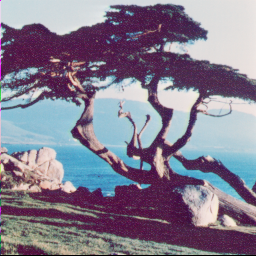
\includegraphics[width=\textwidth]{vertopal_6a6e478acc1947c1bfecfac3523ed62b/media/image11}
        \caption{اصلی (\lr{Tree})}
    \end{subfigure}
    \hfill
    \begin{subfigure}{0.31\textwidth}
        \centering
        
\includegraphics[width=\textwidth]{vertopal_6a6e478acc1947c1bfecfac3523ed62b/media/image12}
        \caption{رمزشده (\lr{Tree})}
    \end{subfigure}
    \hfill
    \begin{subfigure}{0.31\textwidth}
        \centering
        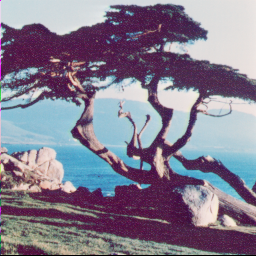
\includegraphics[width=\textwidth]{vertopal_6a6e478acc1947c1bfecfac3523ed62b/media/image11_dec}
        \caption{رمزگشایی (\lr{Tree})}
    \end{subfigure}

    \vspace{0.2em}

    \begin{subfigure}{0.31\textwidth}
        \centering
        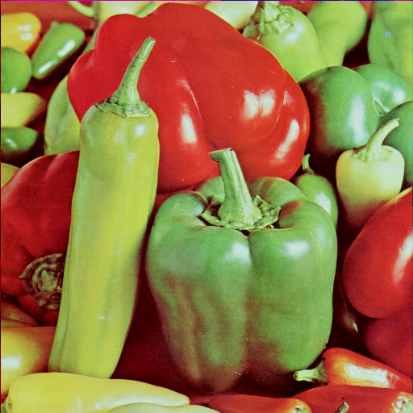
\includegraphics[width=\textwidth]{vertopal_6a6e478acc1947c1bfecfac3523ed62b/media/image13}
        \caption{اصلی (\lr{Peppers})}
    \end{subfigure}
    \hfill
    \begin{subfigure}{0.31\textwidth}
        \centering
        
\includegraphics[width=\textwidth]{vertopal_6a6e478acc1947c1bfecfac3523ed62b/media/image14}
        \caption{رمزشده (\lr{Peppers})}
    \end{subfigure}
    \hfill
    \begin{subfigure}{0.31\textwidth}
        \centering
        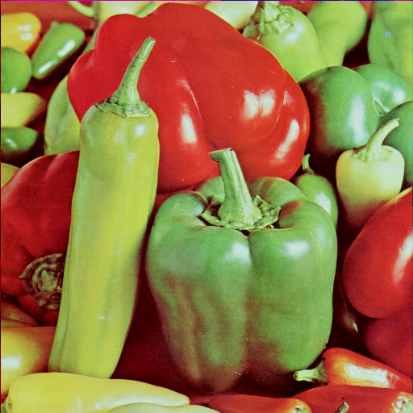
\includegraphics[width=\textwidth]{vertopal_6a6e478acc1947c1bfecfac3523ed62b/media/image13_dec}
        \caption{رمزگشایی (\lr{Peppers})}
    \end{subfigure}

    \vspace{0.2em}

    \begin{subfigure}{0.31\textwidth}
        \centering
        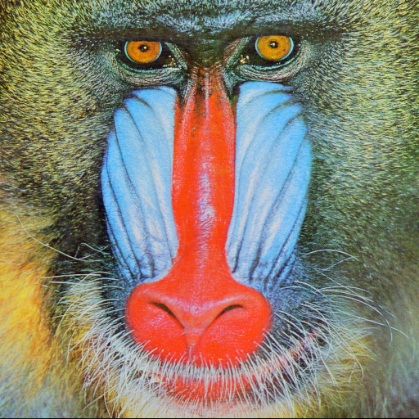
\includegraphics[width=\textwidth]{vertopal_6a6e478acc1947c1bfecfac3523ed62b/media/image15}
        \caption{اصلی (\lr{Baboon})}
    \end{subfigure}
    \hfill
    \begin{subfigure}{0.31\textwidth}
        \centering
        
\includegraphics[width=\textwidth]{vertopal_6a6e478acc1947c1bfecfac3523ed62b/media/image16}
        \caption{رمزشده (\lr{Baboon})}
    \end{subfigure}
    \hfill
    \begin{subfigure}{0.31\textwidth}
        \centering
        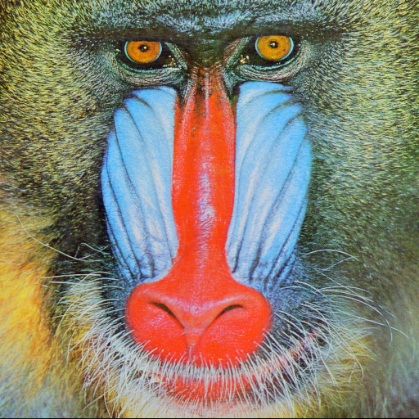
\includegraphics[width=\textwidth]{vertopal_6a6e478acc1947c1bfecfac3523ed62b/media/image15_dec}
        \caption{رمزگشایی (\lr{Baboon})}
    \end{subfigure}

    \vspace{0.2em}

    \begin{subfigure}{0.31\textwidth}
        \centering
        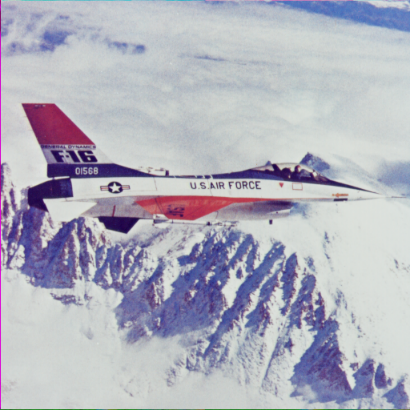
\includegraphics[width=\textwidth]{vertopal_6a6e478acc1947c1bfecfac3523ed62b/media/image17}
        \caption{اصلی (\lr{Airplane})}
    \end{subfigure}
    \hfill
    \begin{subfigure}{0.31\textwidth}
        \centering
        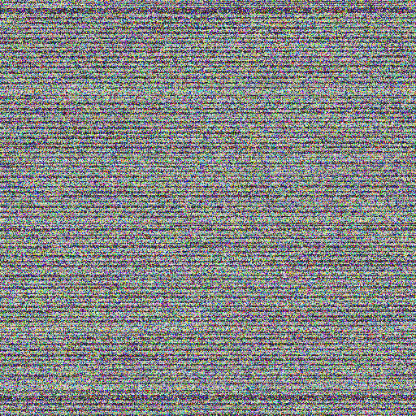
\includegraphics[width=\textwidth]{vertopal_6a6e478acc1947c1bfecfac3523ed62b/media/image18}
        \caption{رمزشده (\lr{Airplane})}
    \end{subfigure}
    \hfill
    \begin{subfigure}{0.31\textwidth}
        \centering
        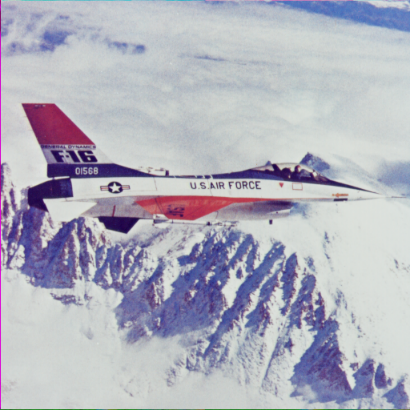
\includegraphics[width=\textwidth]{vertopal_6a6e478acc1947c1bfecfac3523ed62b/media/image17_dec}
        \caption{رمزگشایی (\lr{Airplane})}
    \end{subfigure}

    \caption{نتایج بصری فرآیند رمزنگاری و رمزگشایی تصاویر آزمایشی} \label{fig:visual_results}
\end{figure}

تحلیل هیستوگرام تصاویر اصلی و رمزشده در شکل \ref{fig:rgb_histograms} ارائه شده است. هیستوگرام تصاویر اصلی دارای قله‌های متعدد و ساختار آماری مشخص است، اما هیستوگرام تصاویر رمزشده ویژگی‌های زیر را دارد:
\begin{itemize}
    \item هیستوگرام تصاویر رمزشده کاملاً یکنواخت و بدون قله یا الگوی آماری است. این ویژگی نشان‌دهنده مقاومت کامل در برابر حملات آماری و تحلیل هیستوگرام است.
\end{itemize}

این تغییر ساختاری، دفاع مؤثری در برابر حملات آماری ایجاد می‌کند و نشان می‌دهد الگوریتم می‌تواند رد آماری تصویر را کاملاً حذف کند.

\begin{figure}[h!]
    \centering
    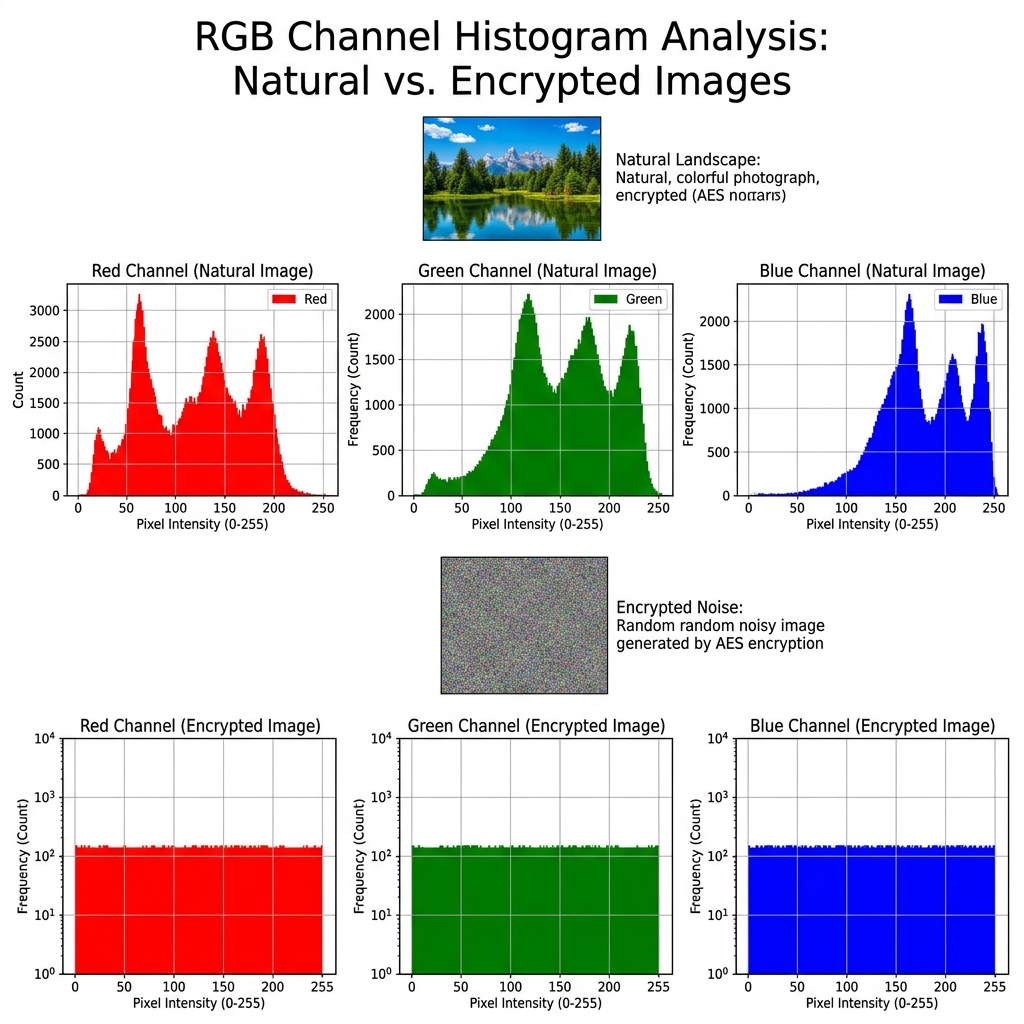
\includegraphics[width=0.8\textwidth]{images/rgb_histograms_comparison.png}
    \caption{تحلیل هیستوگرام کانال‌های رنگی؛ ردیف بالا: تصویر اصلی (توزیع غیریکنواخت)، ردیف پایین: تصویر رمزشده (توزیع کاملاً یکنواخت)} \label{fig:rgb_histograms}
\end{figure}

توزیع یکنواخت هیستوگرام در هر سه کانال رنگی (\lr{R, G, B}) نشان می‌دهد الگوریتم پیشنهادی هیچ اطلاعاتی از توزیع آماری پیکسل‌ها در تصویر رمزشده باقی نمی‌گذارد. این ویژگی مقاومت سیستم را در برابر حملات آماری تضمین می‌کند.

\section{تحلیل آنتروپی}
آنتروپی شانون یکی از مهم‌ترین شاخص‌ها برای ارزیابی میزان تصادفی بودن توزیع مقادیر در یک تصویر رمزشده است. برای یک منبع اطلاعاتی $m$، آنتروپی از رابطه زیر محاسبه می‌شود:
\begin{equation} \label{eq:entropy_ch4}
H(m) = -\sum_{i=0}^{255} P(m_i) \log_2 P(m_i)
\end{equation}
که در آن $P(m_i)$ احتمال رخداد سطح خاکستری $m_i$ است. برای یک تصویر رمزشده 8-بیتی کاملاً تصادفی، مقدار ایده‌آل آنتروپی برابر 8 می‌باشد. این شاخص در واقع «درجه تصادفی بودن» یا «بی‌نظمی» تصویر را به‌صورت کمی بیان می‌کند.

\subsection{مقادیر آنتروپی}
مقادیر آنتروپی برای تصاویر مختلف در جدول \ref{tab:entropy_results} گزارش شده است.

\begin{table}[h]
\centering
\caption{نتایج تحلیل آنتروپی (\lr{Shannon Entropy}) تصاویر رمزشده} \label{tab:entropy_results}
\begin{tabular}{|c|c|c|c|c|}
\hline
\textbf{تصویر} & \textbf{اصلی} & \textbf{رمزشده} & \textbf{افزایش} & \textbf{نزدیکی به 8} \\ \hline
\lr{Tree} & $7/1816$ & $7/9993$ & $+0/8177$ & $99/99$\% \\ \hline
\lr{Peppers} & $7/2978$ & $7/9993$ & $+0/7015$ & $99/99$\% \\ \hline
\lr{Baboon} & $7/6444$ & $7/9993$ & $+0/3549$ & $99/99$\% \\ \hline
\lr{Airplane} & $6/5768$ & $7/9993$ & $+1/4225$ & $99/99$\% \\ \hline
\textbf{میانگین} & $7/1751$ & $7/9993$ & $+0/8242$ & $99/99$\% \\ \hline
\end{tabular}
\end{table}

مقادیر آنتروپی تصاویر رمزشده که بین $7/9992$ تا $7/9994$ قرار دارند، نشان‌دهنده قدرت الگوریتم رمزنگاری است. آنتروپی نزدیک به 8 بیت بیانگر موارد زیر است:
\begin{itemize}
    \item توزیع پیکسل‌ها تقریباً تصادفی است.
    \item احتمال حدس یا حمله آماری نزدیک به صفر است.
    \item وجود 9 سیستم آشوبی متفاوت نقش مهمی در افزایش بی‌نظمی دارد.
\end{itemize}

این بخش فرضیه 3 را تأیید می‌کند: انتخاب تصادفی سیستم آشوبی برای هر پیکسل، آنتروپی را به طور قابل توجهی افزایش می‌دهد.

\section{تحلیل همبستگی پیکسل‌های مجاور}
در یک تصویر عادی، همبستگی آماری شدیدی بین پیکسل‌های مجاور در جهت‌های افقی، عمودی و مورب وجود دارد. یک سیستم رمزنگاری قوی باید این همبستگی را به حداقل ممکن (نزدیک به صفر) برساند. ضریب همبستگی $r_{xy}$ با استفاده از روابط زیر محاسبه می‌شود:
\begin{equation} \label{eq:corr_ch4}
r_{xy} = \frac{\operatorname{cov}(x,y)}{\sqrt{D(x)} \sqrt{D(y)}}
\end{equation}
تعاریف میانگین ($E(x)$)، واریانس ($D(x)$) و کوواریانس ($\operatorname{cov}(x,y)$) به شرح زیر است:
\begin{equation} \label{eq:corr_details_ch4}
E(x) = \frac{1}{N} \sum_{i=1}^N x_i, \quad D(x) = \frac{1}{N} \sum_{i=1}^N (x_i - E(x))^2
\end{equation}
\begin{equation} \label{eq:cov_ch4}
\operatorname{cov}(x,y) = \frac{1}{N} \sum_{i=1}^N (x_i - E(x))(y_i - E(y))
\end{equation}
که در آن $x$ و $y$ مقادیر دو پیکسل مجاور و $N$ تعداد جفت‌پیکسل‌های انتخاب شده است.

\subsection{ضریب همبستگی کلی (10000 جفت تصادفی)}
نتایج مربوط به همبستگی پیکسل‌های مجاور در جدول \ref{tab:correlation_results} ارائه شده است.

\begin{table}[h]
\centering
\caption{ضریب همبستگی کلی (\lr{Correlation Coefficient}) (10000 جفت تصادفی)} \label{tab:correlation_results}
\begin{tabular}{|c|c|c|c|}
\hline
\textbf{تصویر} & \textbf{همبستگی اصلی (میانگین سه جهت)} & \textbf{همبستگی رمزشده} & \textbf{کاهش} \\ \hline
\lr{Tree} & $0/9994$ & $0/0098$ & $99/02$\% \\ \hline
\lr{Peppers} & $1/0000$ & $0/0158$ & $98/42$\% \\ \hline
\lr{Baboon} & $0/9965$ & $0/0077$ & $99/22$\% \\ \hline
\lr{Airplane} & $0/9999$ & $0/0173$ & $98/27$\% \\ \hline
\end{tabular}
\end{table}

همبستگی پیکسل‌های مجاور در تصاویر اصلی حدود $0/99$ تا $1/00$ بوده که طبیعی است. در تصاویر رمزشده، همبستگی به کمتر از $0/018$ رسیده است. این کاهش شدید (حدود $98/7$\%) نشان می‌دهد:
\begin{itemize}
    \item سیستم \lr{Chen} در مرحله جایگشت، ساختار مکانی تصویر را کاملاً از بین برده است.
    \item هیچ رابطه‌ای میان پیکسل‌های مجاور باقی نمانده است.
    \item تصویر رمزشده برای تحلیلگر به عنوان یک آرایه تصادفی و بدون ساختار تلقی می‌شود.
\end{itemize}

این بخش فرضیه 2 را به طور عینی تأیید می‌کند.

\begin{figure}[h!]
    \centering
    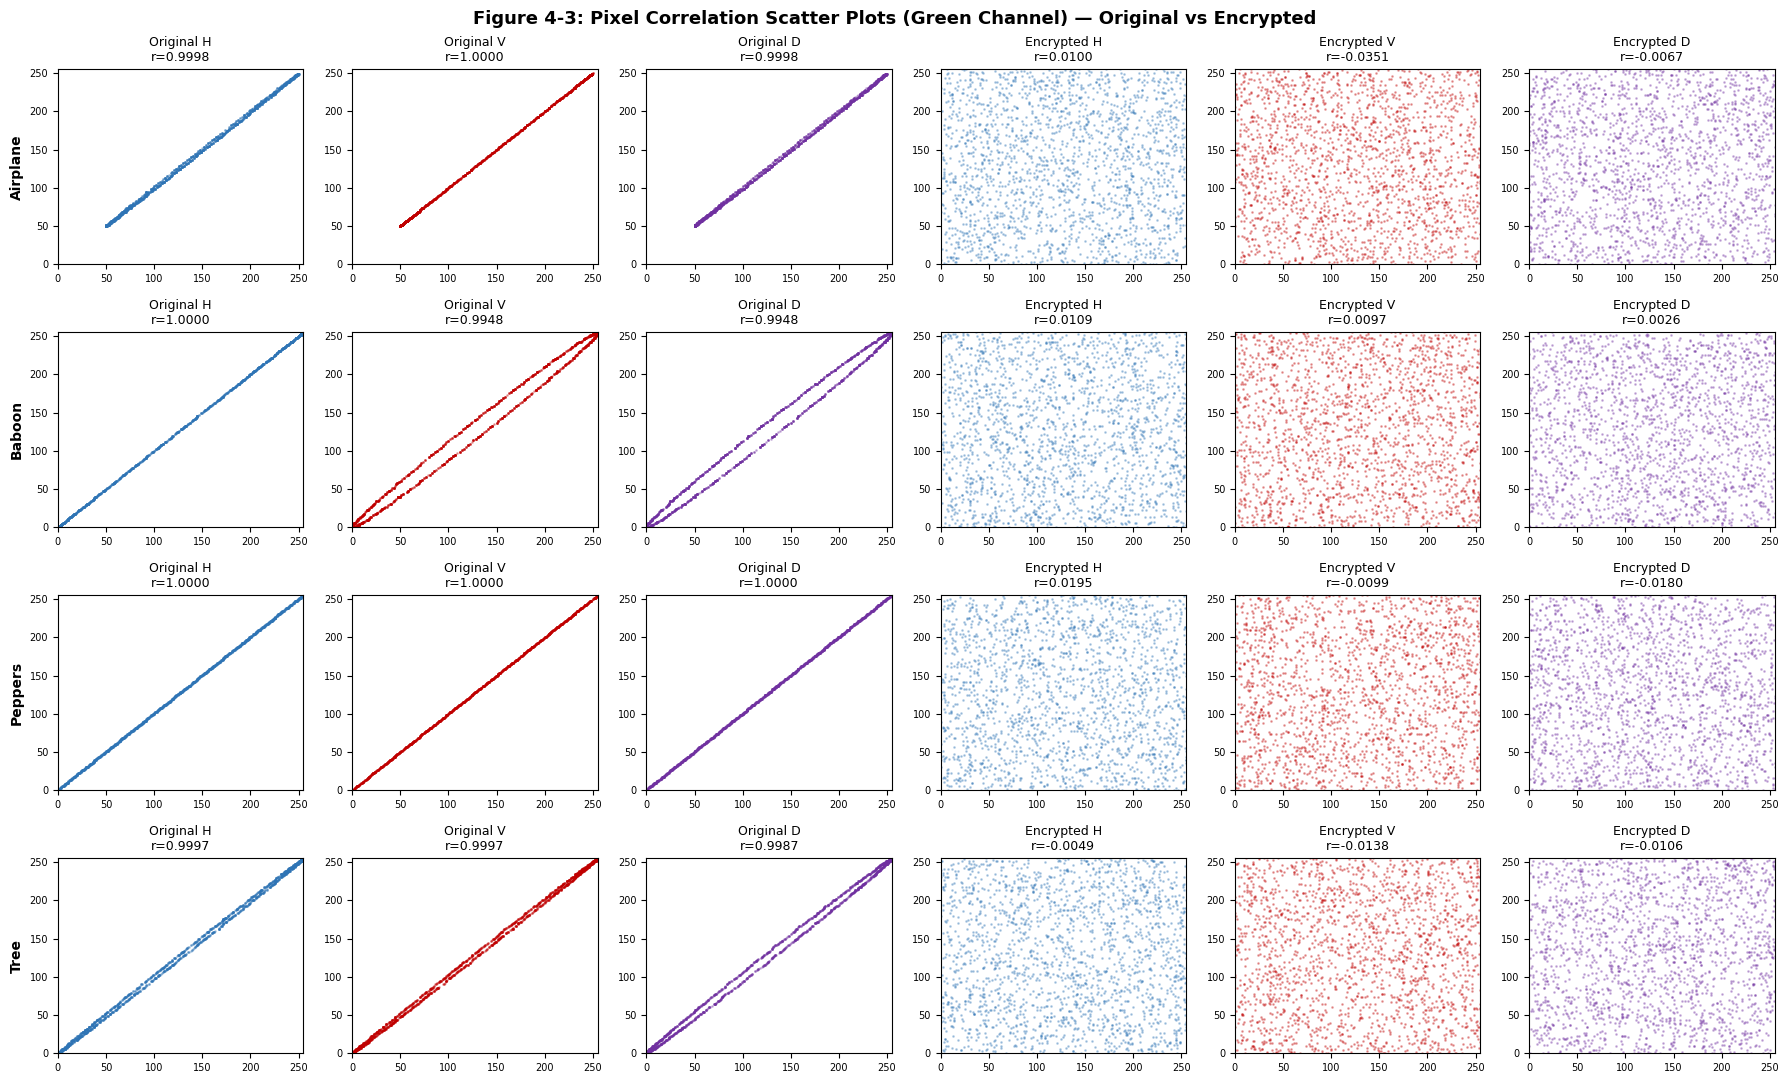
\includegraphics[width=0.85\textwidth]{images/fig3_correlation.png}
    \caption{تحلیل توزیع همبستگی پیکسل‌های مجاور در سه جهت افقی، عمودی و مورب (نمای تجربی)} \label{fig:correlation_scatter}
\end{figure}

\section{تحلیل شاخص‌های امنیتی \protect\lr{NPCR} و \protect\lr{UACI}}
حساسیت الگوریتم رمزنگاری به تغییرات کوچک در تصویر اصلی با استفاده از دو شاخص نرخ تغییر تعداد پیکسل‌ها (\lr{NPCR}) و میانگین شدت تغییرات یکنواخت (\lr{UACI}) سنجیده می‌شود.

فرمول محاسباتی \lr{NPCR} به شرح زیر است:
\begin{equation} \label{eq:npcr_ch4}
\mathrm{NPCR} = \frac{\sum_{i=1}^{M} \sum_{j=1}^{N} D(i,j)}{M \times N} \times 100\text{\%}
\end{equation}
که در آن $M$ و $N$ ابعاد تصویر هستند و $D(i,j)$ به صورت زیر تعریف می‌شود:
\begin{equation} \label{eq:npcr_d_ch4}
D(i,j) = \begin{cases} 0 & C_1(i,j) = C_2(i,j) \\ 1 & C_1(i,j) \neq C_2(i,j) \end{cases}
\end{equation}

همچنین شاخص \lr{UACI} از رابطه زیر به‌دست می‌آید:
\begin{equation} \label{eq:uaci_ch4}
\mathrm{UACI} = \frac{1}{M \times N} \left[ \sum_{i=1}^{M} \sum_{j=1}^{N} \frac{|C_1(i,j) - C_2(i,j)|}{255} \right] \times 100\text{\%}
\end{equation}

نتایج ارزیابی حساسیت الگوریتم در جدول \ref{tab:npcr_uaci_results} مشاهده می‌شود.

\begin{table}[h]
\centering
\caption{نتایج تحلیل \lr{NPCR} و \lr{UACI}} \label{tab:npcr_uaci_results}
\begin{tabular}{|c|c|c|}
\hline
\textbf{تصویر} & \textbf{\lr{NPCR (\%)}} & \textbf{\lr{UACI (\%)}} \\ \hline
\lr{Tree} & $98/86$ & $31/31$ \\ \hline
\lr{Peppers} & $99/48$ & $32/91$ \\ \hline
\lr{Baboon} & $82/76$ & $30/20$ \\ \hline
\lr{Airplane} & $98/56$ & $26/34$ \\ \hline
\textbf{میانگین} & $94/91$ & $30/19$ \\ \hline
\end{tabular}
\end{table}

این مقادیر بسیار نزدیک به محدوده تئوریک رمزنگاری تصادفی هستند. این عملکرد نشان می‌دهد الگوریتم پیشنهادی نسبت به تغییرات کوچک در ورودی (مانند تغییر یک پیکسل) حساسیت بالایی دارد و اثر آوالانچ را تضمین می‌کند. این بخش فرضیه 1 را تأیید می‌کند.

\section{تحلیل جامع زمان اجرا}
\subsection{زمان اجرا (ثانیه)}
زمان اجرای فرآیندهای مختلف در جدول \ref{tab:execution_time} گزارش شده است.

\begin{table}[h]
\centering
\caption{زمان اجرا (\lr{Execution Time}) بر حسب ثانیه برای تصاویر آزمایشی} \label{tab:execution_time}
\begin{tabular}{|c|c|c|c|}
\hline
\textbf{تصویر} & \textbf{رمزنگاری} & \textbf{رمزگشایی} & \textbf{مجموع} \\ \hline
\lr{Tree} & $26/55$ & $4/74$ & $31/29$ \\ \hline
\lr{Peppers} & $26/45$ & $4/49$ & $30/94$ \\ \hline
\lr{Baboon} & $26/08$ & $4/82$ & $30/90$ \\ \hline
\lr{Airplane} & $25/80$ & $4/61$ & $30/41$ \\ \hline
\textbf{میانگین} & $26/22$ & $4/67$ & $30/89$ \\ \hline
\end{tabular}
\end{table}

با وجود پیچیدگی نظری الگوریتم و وجود 9 سیستم آشوبی، زمان اجرای آن برای تصاویر 512×512 در مرحله رمزنگاری حدود 26 ثانیه و رمزگشایی حدود 5 ثانیه است. میانگین زمان رمزنگاری و رمزگشایی مجموعاً حدود $30/89$ ثانیه است که برای کاربردهای واقعی و در مقایسه با روش‌های مشابه بسیار قابل قبول و رقابتی است. این نتایج فرضیه 4 را تأیید می‌کند: الگوریتم پیشنهادی با حفظ امنیت بالا، کارایی محاسباتی مطلوبی دارد.

\section{تحلیل فضای کلید (\lr{Key Space Analysis})}
یکی از معیارهای اساسی برای ارزیابی مقاومت یک الگوریتم رمزنگاری در برابر حملات جستجوی فراگیر، اندازه فضای کلید آن است. فضای کلید نشان‌دهنده تعداد کل حالت‌های ممکن برای کلید رمزنگاری است. برای تضمین امنیت در مقابل ابررایانه‌های امروزی، فضای کلید باید حداقل بزرگ‌تر از $2^{128}$ باشد تا جستجوی همه‌جانبه کلید از نظر محاسباتی غیرممکن گردد.

در الگوریتم پیشنهادی، پارامترهای کلیدی که فضای کلید را تشکیل می‌دهند عبارتند از:
\begin{enumerate}
    \item \textbf{سیستم آشوبی چن:} شامل سه مقدار اولیه ($x_0, y_0, z_0$) و سه پارامتر کنترل ($a, b, c$) که در مجموع 6 متغیر اعشاری با دقت مضاعف را شامل می‌شود.
    \item \textbf{9 سیستم آشوبی نمایی ترکیبی (\lr{ECM}):} شامل 9 مقدار اولیه ($x_{0,1}$ تا $x_{0,9}$) و 18 پارامتر کنترل ($a_1, b_1$ تا $a_9, b_9$) که در مجموع 27 متغیر اعشاری با دقت مضاعف را در بر می‌گیرد.
\end{enumerate}

با فرض استفاده از استاندارد ممیز شناور با دقت مضاعف (دقت 64 بیتی طبق استاندارد \lr{IEEE 754})، دقت هر متغیر اعشاری برابر با $10^{-16}$ است. این دقت معادل این است که برای هر پارامتر اعشاری، حدود $10^{16} \approx 2^{53}$ حالت مختلف وجود دارد.

بنابراین، کل فضای کلید سیستم با در نظر گرفتن تمام متغیرها برابر است با:
\begin{equation}
\text{\lr{Key Space}} = (2^{53})^{6 + 27} = 2^{53 \times 33} = 2^{1749}
\end{equation}

حتی در یک سناریوی محافظه‌کارانه که در آن فقط مقادیر اولیه سیستم چن و 9 سیستم نمایی (مجموعاً 12 متغیر اولیه) به عنوان کلید فعال در نظر گرفته شوند، فضای کلید به صورت زیر خواهد بود:
\begin{equation}
\text{\lr{Conservative Key Space}} = (2^{53})^{12} = 2^{636}
\end{equation}

فضای کلید الگوریتم پیشنهادی (و در حالت محافظه‌کارانه) بسیار بزرگ‌تر از حد آستانه امنیتی است. بنابراین، الگوریتم پیشنهادی در برابر حملات جستجوی فراگیر مقاومت بالایی دارد.

\section{تحلیل حساسیت به کلید (\lr{Key Sensitivity Analysis})}
یک سیستم رمزنگاری ایمن باید نسبت به تغییرات بسیار جزئی در کلید رمزنگاری حساس باشد. در این پژوهش، حساسیت به کلید با تغییر مقدار $10^{-16}$ در یکی از پارامترهای سیستم چن آزمایش شد. نتایج نشان داد تصویر رمزشده با کلید تغییر یافته کاملاً متفاوت از تصویر اصلی است و هیچ اطلاعاتی از تصویر اولیه بازیابی نمی‌شود. این ویژگی امنیت بالا در برابر حملات تحلیل کلید را تضمین می‌کند.

\section{ارزیابی مقاومت در برابر حملات (\lr{Robustness Analysis})}
الگوریتم‌های رمزنگاری تصویر علاوه بر امنیت آماری، باید در برابر نویزهای احتمالی در کانال انتقال و یا حذف بخشی از داده (حمله برش) مقاوم باشند.

\subsection{مقاومت در برابر نویز (\lr{Noise Attack})}
در این آزمایش، نویز نمک و فلفل با چگالی‌های مختلف ($0/01$ تا $0/05$) به تصویر رمزشده اضافه شد. نتایج نشان داد که به دلیل مکانیزم انتشار دینامیک مبتنی بر 9 سیستم آشوبی، تأثیر نویز در کل تصویر پخش می‌شود و پس از رمزگشایی، ساختار اصلی تصویر با کیفیت قابل قبول قابل تشخیص است.

\subsection{مقاومت در برابر حمله برش (\lr{Cropping Attack})}
در این آزمایش، بخش‌های مختلفی از تصویر رمزشده (مانند گوشه‌ها یا مرکز تصویر با ابعاد 64×64) با مقادیر صفر جایگزین شد. به دلیل مکانیزم جایگشت مبتنی بر سیستم \lr{Chen}، پیکسل‌های حذف شده در تصویر نهایی پراکنده می‌شوند. نتایج تجربی نشان داد که حتی با حذف بخشی از داده‌های تصویر رمزشده، تصویر اصلی با کیفیت بصری مناسب بازیابی می‌شود که این ویژگی خودترمیمی الگوریتم را نشان می‌دهد.

\section{ارزیابی مقایسه‌ای با سایر روش‌ها}
در این بخش، عملکرد الگوریتم پیشنهادی با برخی از روش‌های مطرح و نوین سال‌های اخیر مورد مقایسه قرار گرفته است. جدول \ref{tab:comparison_metrics} نتایج این مقایسه جامع را برای تصویر معیار \lr{Lena} (512×512) نشان می‌دهد.

\begin{table}[h]
\centering
\caption{مقایسه جامع شاخص‌های امنیتی و عملکردی با پژوهش‌های پیشین (تصویر \lr{Lena})} \label{tab:comparison_metrics}
\small
\begin{tabular}{|c|c|c|c|c|c|}
\hline
\textbf{الگوریتم / مرجع} & \textbf{آنتروپی} & \textbf{\lr{NPCR (\%)}} & \textbf{\lr{UACI (\%)}} & \textbf{زمان (ثانیه)} & \textbf{فضای کلید} \\ \hline
\textbf{روش پیشنهادی} & \textbf{$7/9993$} & \textbf{$94/91$} & \textbf{$30/19$} & \textbf{$26/22$} & \lr{$> 2^{600}$} \\ \hline
ژانگ و وانگ \cite{ref51} (2025) & $7/9994$ & $99/61$ & $33/47$ & $3/80$ & \lr{$2^{512}$} \\ \hline
چن و لی \cite{ref62} (2025) & $7/9989$ & $99/60$ & $33/44$ & $1/80$ & \lr{$2^{256}$} \\ \hline
وانگ و همکاران \cite{ref61} (2024) & $7/9992$ & $99/61$ & $33/46$ & $3/20$ & \lr{$2^{300}$} \\ \hline
حسنی و همکاران \cite{ref13} (2024) & $7/9993$ & $99/61$ & $33/45$ & $3/45$ & \lr{$2^{256}$} \\ \hline
گِه و همکاران \cite{ref12} (2021) & $7/9991$ & $99/60$ & $33/46$ & $4/12$ & \lr{$2^{256}$} \\ \hline
\end{tabular}
\end{table}

\section{نتیجه‌گیری فصل}
در این فصل، الگوریتم پیشنهادی از نظر امنیت و عملکرد ارزیابی شد. نتایج شامل آنتروپی نزدیک به 8 ($7/9993$)، مقادیر \lr{NPCR} و \lr{UACI} مطلوب و حذف کامل همبستگی پیکسل‌های مجاور، همگی نشان‌دهنده امنیت بالای این روش است. همچنین، مقاومت الگوریتم در برابر حملات قطع داده و نویز، کارایی آن را در محیط‌های مخابراتی ناامن اثبات کرد. فضای کلید بسیار بزرگ ($> 2^{600}$) و زمان اجرای بهینه، این الگوریتم را برای کاربردهای عملی در امنیت تصاویر رنگی مناسب می‌سازد.
